\chapter{Mathematical and Numerical Robustness}

The mathematical and numerical robustness of a deterministic computer model depends upon 
three issues: the code must be transparent so that it can be understood and modified by visual 
inspection; it must be possible to check and verify with automated tools; and there must be a 
method for checking the correctness of the solution, at least for asymptotic (steady state) 
solutions (numerical stability and agreement with known solutions). 

In order to understand the meaning of accuracy and robustness, it is necessary to understand the 
means by which the numerical routines are structured. In this chapter, details of the 
implementation of the model are presented, including the tests used to assess the numerical 
aspects of the model.  These include 

\begin{itemize}
\item the structure of the model, including the major routines implementing the various 
physical phenomena included in the model, 
\item the organization of data initialization and data input used by the model, 
\item the structure of data used to formulate the differential equations solved by the model, 
\item a summary of the main control routines in the model that are used to control all input and 
output, initialize the model and solve the appropriate differential equation set for the 
problem to be solved, 
\item the means by which the computer code is checked for consistency and correctness, 
\item analysis of the numerical implementation for stability and error propagation, and 
\item comparison of the results of the system model with simple analytical or numerical 
solutions. 
\end{itemize}

\section{Structure of the Numerical Routines}
\label{sec:Subroutines}

A methodology which is critical to verification of the model is the schema used to incorporate 
physical phenomena. This is the subroutine structure discussed below. The method for 
incorporating new phenomena and insuring the correctness of the code was adopted as part of 
the consolidation of CCFM and FAST. This consolidation occurred in 1990 and has resulted in a 
more transparent, transportable and verifiable numerical model. This transparency is crucial to a 
verifiable and robust numerical implementation of the predictive model as discussed in the 
sections on code checking and numerical analysis.

The model can be split into distinct parts.  There are routines for reading data, calculating results 
and reporting the results to a file or printer.  The major routines for performing these functions 
are identified in figure \ref{fig:Subroutines}.  These physical interface routines link the CFAST model to the actual routines which calculate quantities such as mass or energy flow at one particular point in time 
for a given environment. 

\begin{figure}
\begin{center}
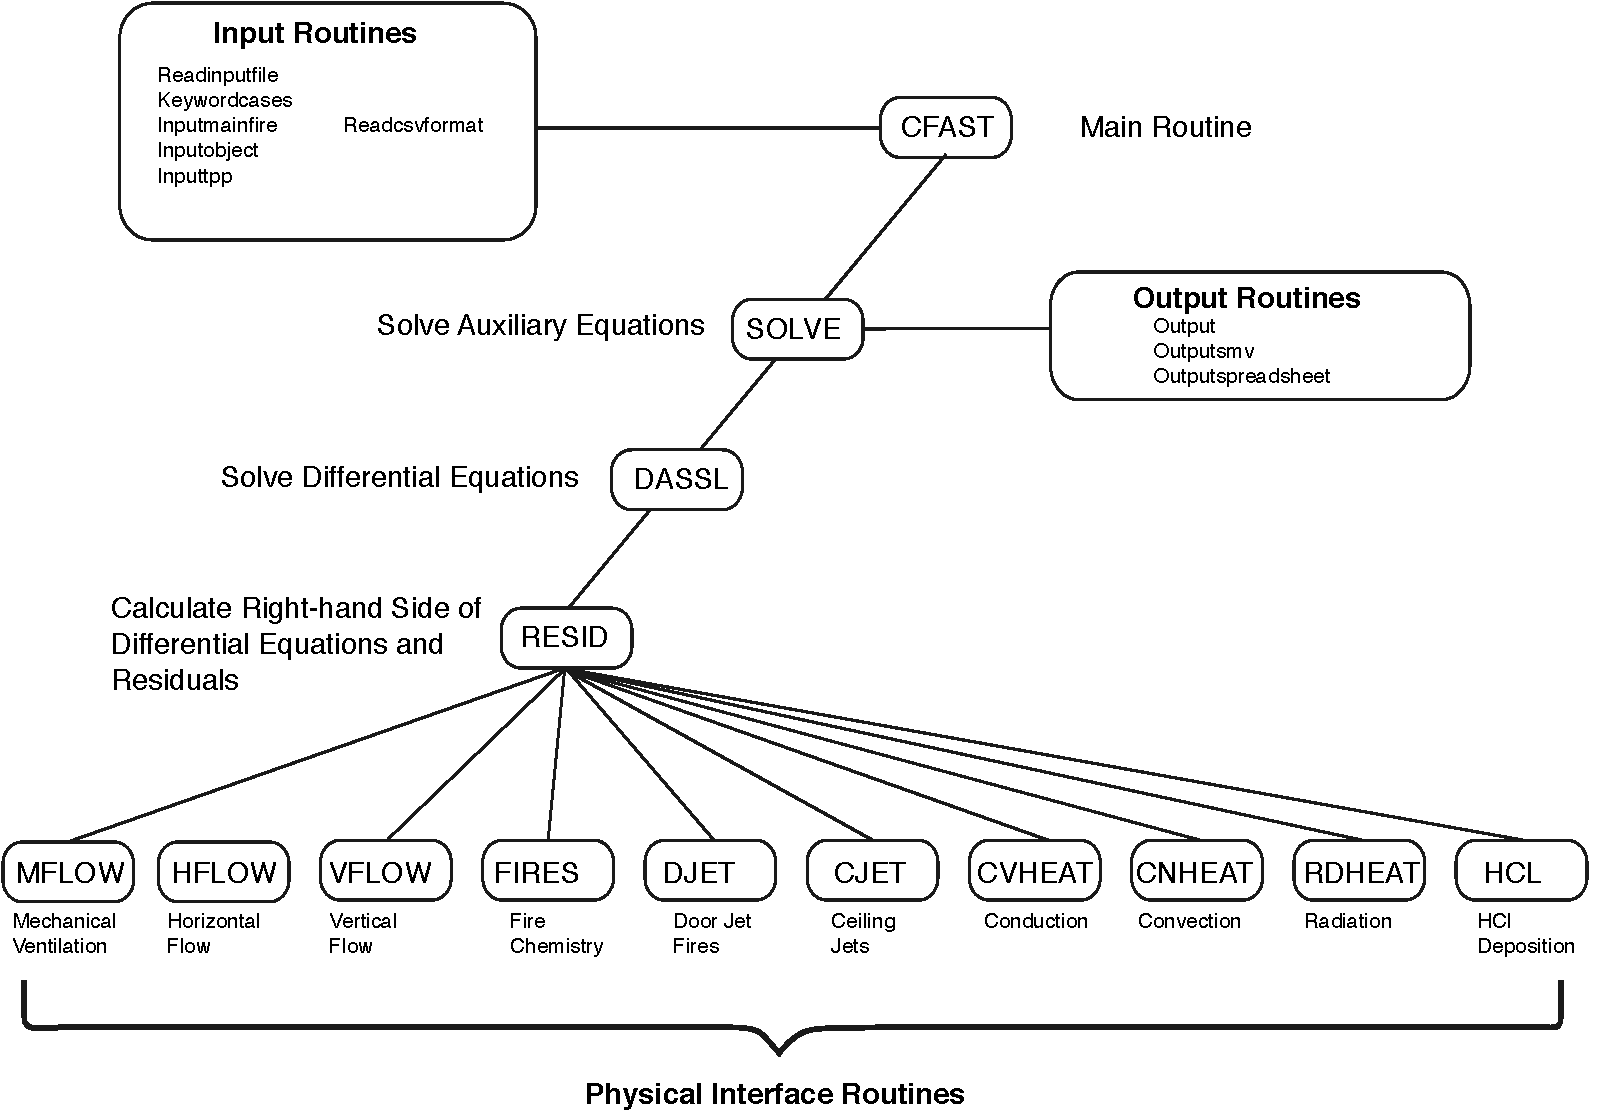
\includegraphics[width=6.4in]{FIGURES/Robustness/Structure}\\
\end{center}
\caption{Subroutine structure for the CFAST model.}
 \label{fig:Subroutines}
\end{figure}

The routines SOLVE, RESID and DASSL are the key to understanding how the physical 
equations are solved.  SOLVE is the control program that oversees the general solution of the 
problem.  It invokes the differential equation solver DASSL \cite{DASSL} which in turn calls RESID to 
solve the transport equations.  Given a solution at time $t$, what is the solution at time t plus a 
small increment of time, $\Delta t$, (where the time increment is determined dynamically by the 
program to insure convergence of the solution at $t + \Delta t$)?  The differential equations are of the 
form 

\be
\frac{dy}{dt} = f(y,t) \; , \; y(t_0) = y_0
\label{eq:basicsolution}
\ee
where $y$ is a vector representing pressure, layer height, mass and such, and $f$ is a vector function
that represents changes in these values with respect to time.  The term $y_0$ is an initial condition at 
the initial time $t_0$ .  The subroutine RESID computes the right hand side of eq (\ref{eq:basicsoultion}) and returns a set of residuals of that calculation to be compared to the values expected by DASSL.  DASSL then checks for convergence.  Once DASSL reaches an error limit (defined as convergence of 
the equations) for the solution at $t + \Delta t$,  SOLVE then advances the solution of species concentra- 
tion, wall temperature profiles, and mechanical ventilation for the same time interval. 
Note that there are several distinct time scales that are involved in the solution of this type of 
problem.  The fastest will be chemical kinetics.  We avoid that scale by assuming that the 
chemistry is infinitely fast.  The next larger time scale is that associated with the flow field. 
These are the equations which are cast into the form of ordinary differential equations.  Then 
there is the time scale for mechanical ventilation, and finally, heat conduction through objects. 
Chemical kinetic times are typically on the order of milliseconds.  The transport time scale are 
on the order of 0.1 s.  The mechanical ventilation and conduction time scales are typically 
several seconds, or even longer.  The time step is dynamically adjusted to a value appropriate for 
the solution of the currently defined equation set.  In addition to allowing a more correct solution 
to the pressure equation, very large time steps are possible if the problem being solved 
approaches steady-state.

\section{Code Checking}

There are two means to automate checking the correctness of the language used by a numerical 
model. The first is the use of standard methods for checking the structure and interface. 
Programs such as Flint and Lint are standard tools to do such checking. They are applied to the 
whole model. There are three aspects of the model checked by this procedure: correctness of the 
interface, undefined or incorrectly defined (or used) variables and constants, and completeness 
of loops and threads. It does not check for the correctness of the numerical use of constants or 
variables only that they are used correctly in a syntactical sense. Lint is part of most C language 
distributions of Unix. Flint is the equivalent for the FORTRAN language. Though it is not 
usually included with FORTRAN distributions Flint is generally available \footnote{Cleanscape Software, 445 Sherman Ave, Ste. Q, Palo Alto, CA 94306}. Both have been used with CFAST. 

The second is to use a variety of computer platforms to compile and run the code. Since 
FORTRAN and C are implemented differently for various computers, this represents both a 
numerical check as well as a syntactic check. CFAST has been compiled for the Sun (Solaris), 
SGI (Irix), the windows-based PCs (Lahey, Digital, and Intel FORTRAN), and the Concurrent 
Computer platforms. Within the precision afforded by the various hardware implementations, the 
answers are identical \footnote{Typically one part in 10\superscript{-6}, which is the error limit used for DASSL.}.

\section{Numerical Tests}

There are two components to testing the numerical solutions of CFAST.  First, the DASSL 
solver is well tested for a wide variety of differential equations, and is widely used and accepted 
\cite{DASSL}. Also, the radiation and conduction routines are tested with known solutions. These are not 
analytical tests, but physical limits, such as an object immersed in a fluid of constant 
temperature, to which the temperature must equilibrate. The solver(s) must show that the 
differential equations asymptotically converge to these answers. 

The second is to insure that the coupling between algorithms and the solver is correct. Most 
errors are avoided because of the structure discussed in section \ref{sec:Subroutines}. The error due to the numerical solution is far less than that associated with the model assumptions. Two examples of 
this are the coupling of mechanical ventilation with buoyant flow, and the Nusselt number 
assumption for boundary layer convection. For the former, the coupling of a network of 
incompressible flow with an ODE for compressible flow has to deal with disparate calculations 
of pressure. For the latter, a very small time step occurs when a floor is heated and the thermal 
wave reaches the far (unexposed) side. This is a limitation of the physical implementation of the 
heat flow algorithm (convection). The solver arrives at the correct solution, but the time step 
becomes very small in order to achieve this. 

Numerical error can be divided into three categories: roundoff, truncation and discretization 
error. Roundoff error occurs because computers represent real numbers using a finite number of 
digits. Truncation error occurs when an infinite process is replaced by a finite one. This can 
happen, for example, when an in finite series is truncated after a finite number of terms or when 
an iteration is terminated after a convergence criterion has been satisfied. Discretization error 
occurs when a continuous process such as a derivative is approximated by a discrete analog such 
as a divided difference. CFAST is designed to use 64-bit precision for real number calculations 
to minimize these effects. 

Implicit in solving the equations discussed in chapter \ref{sec:Theory_Chapter}, is that the solver will arrive at a solution.  Inherent in the DASSL solver are convergence criteria for the mass and energy balance within CFAST to insure mass and energy conservation within 1 part in 10\superscript{6}.  There are, however, limitations introduced by the algorithmic realization of physical models, that can produce errors and instabilities. Using the example above, if a mechanical ventilation system injects or removes 
mass and enthalpy from a small duct, then there can be a stability issue with the layer interface 
bobbing up and down over the duct. These are annoyances to the user community and 
shortcomings of the implementation of algorithm rather than failure of the system model.

Problems of this sort are noted in the �frequently asked questions� on the CFAST web site 
(http://cfast.nist.gov).

\section{Comparison with Analytic Solutions}

There do not exist general analytic solutions for fire problems, even for the simplest cases. That 
is, there are no closed form solutions to this type of problem. However, it is possible to do two 
kinds of checking. The first type is discussed in the section on the theoretical basis of the model, 
for which individual algorithms are validated against experimental work. The second is simple 
experiments, especially for conduction and radiation, for which the results are asymptotic. For 
example, for a simple, single compartment test case with no fire, all temperatures should 
equilibrate asymptotically to a single value.  Such comparisons are common and not usually 
published.